\section{Ferramentas e Datasets}

\begin{frame}{Ferramentas e Datasets}
    Você já viu o pipeline inteiro: descoberta, identificação, estimação, refutação.

    \pause
    \vfill
    Pergunta que todo mundo faz depois de um curso de causalidade: \textbf{``beleza, mas eu clico em quê pra fazer isso?''}

    \begin{figure}
        \centering
        
\includegraphics[width=0.2\linewidth]{figures/nazare.jpg}
    \end{figure}
\end{frame}

\begin{frame}[plain]
    \begin{table}[htbp]
    \centering
    \label{tab:causal_tools}
    \small
    \begin{tabular}{lccccc}
    \toprule
    \textbf{Ferramenta} & \textbf{Descoberta} & \textbf{Estimação} & \textbf{Refutação} & \textbf{Interface} & \textbf{Paralelo} \\
    \midrule
    CDT \cite{tool-causaldiscoverytoolbox} & \checkmark & -- & -- & -- & -- \\
    causal-learn \cite{tool-causallearn} & \checkmark & -- & -- & -- & -- \\
    bnlearn \cite{tool-bnlearn} & \checkmark & -- & -- & -- & -- \\
    Tetrad \cite{tool-tetrad} & \checkmark & -- & -- & \checkmark & -- \\
    gCastle \cite{tool-gcastle} & \checkmark & -- & -- & -- & -- \\
    DoWhy \cite{ai-sharma2020dowhy} & -- & \checkmark & \checkmark & -- & -- \\
    EconML \cite{tool-econml} & -- & \checkmark & -- & -- & -- \\
    CausalML \cite{ai-chen2020causalml} & -- & \checkmark & -- & -- & \checkmark \\
    CausalNex \cite{tool-causalnex} & \checkmark & \checkmark & -- & -- & -- \\
    Salesforce CausalAI \cite{tool-salesforce-causalai} & \checkmark & -- & -- & \checkmark & \checkmark \\
    \textit{Causal-Nest} \cite{causal-nest-kbs} & \checkmark & \checkmark & \checkmark & -- & \checkmark \\
    \bottomrule
    \end{tabular}
    \end{table}
\end{frame}

\begin{frame}{Ferramentas}{Um problema meio óbvio}
    Repara no padrão da tabela: \pause praticamente ninguém faz tudo.

    \pause
    \begin{itemize}
        \item Ferramentas de \textbf{descoberta} (CDT, causal-learn, bnlearn, Tetrad, gCastle) sabem achar a estrutura, mas não estimam nem refutam nada;
        \pause
        \item Ferramentas de \textbf{inferência} (DoWhy, EconML, CausalML) já assumem que você chegou com um grafo pronto na mão.
        \item Alguns backends em R; as representações de grafo são diferentes, etc.
    \end{itemize}

    \pause
    \vfill
    Na prática, isso significa juntar ferramentas diferentes manualmente: converter formato de dado, e torcer pra estrutura descoberta bater com o que a ferramenta de inferência espera.

    \pause
    \vfill
    O \textit{Causal-Nest} (projeto do autor) é uma tentativa de unificar esse pipeline inteiro numa única interface.
\end{frame}

\begin{frame}{Datasets}{Onde está o gabarito?}
    Em ML supervisionado, você tem o rótulo verdadeiro pra comparar. Em CD, isso quase nunca acontece: o grafo causal ``de verdade'' por trás de um dataset observacional raramente é conhecido com certeza.

    \pause
    \vfill
    O \textbf{Sachs}, que a gente usou lá no Notebook 2, é a exceção rara: um dos poucos datasets reais com grafo verdadeiro validado por experimentos de intervenção de verdade.

    \pause
    \vfill
    A grande maioria dos outros benchmarks conhecidos não tem um grafo completo. Eles trazem, no máximo, pistas parciais: ordem temporal entre variáveis, ou uma lista de arestas proibidas e obrigatórias.
\end{frame}

\begin{frame}{O ``Expert'' no meio do pipeline?}
    Lembra dessa figura?

    \begin{figure}
        \centering
        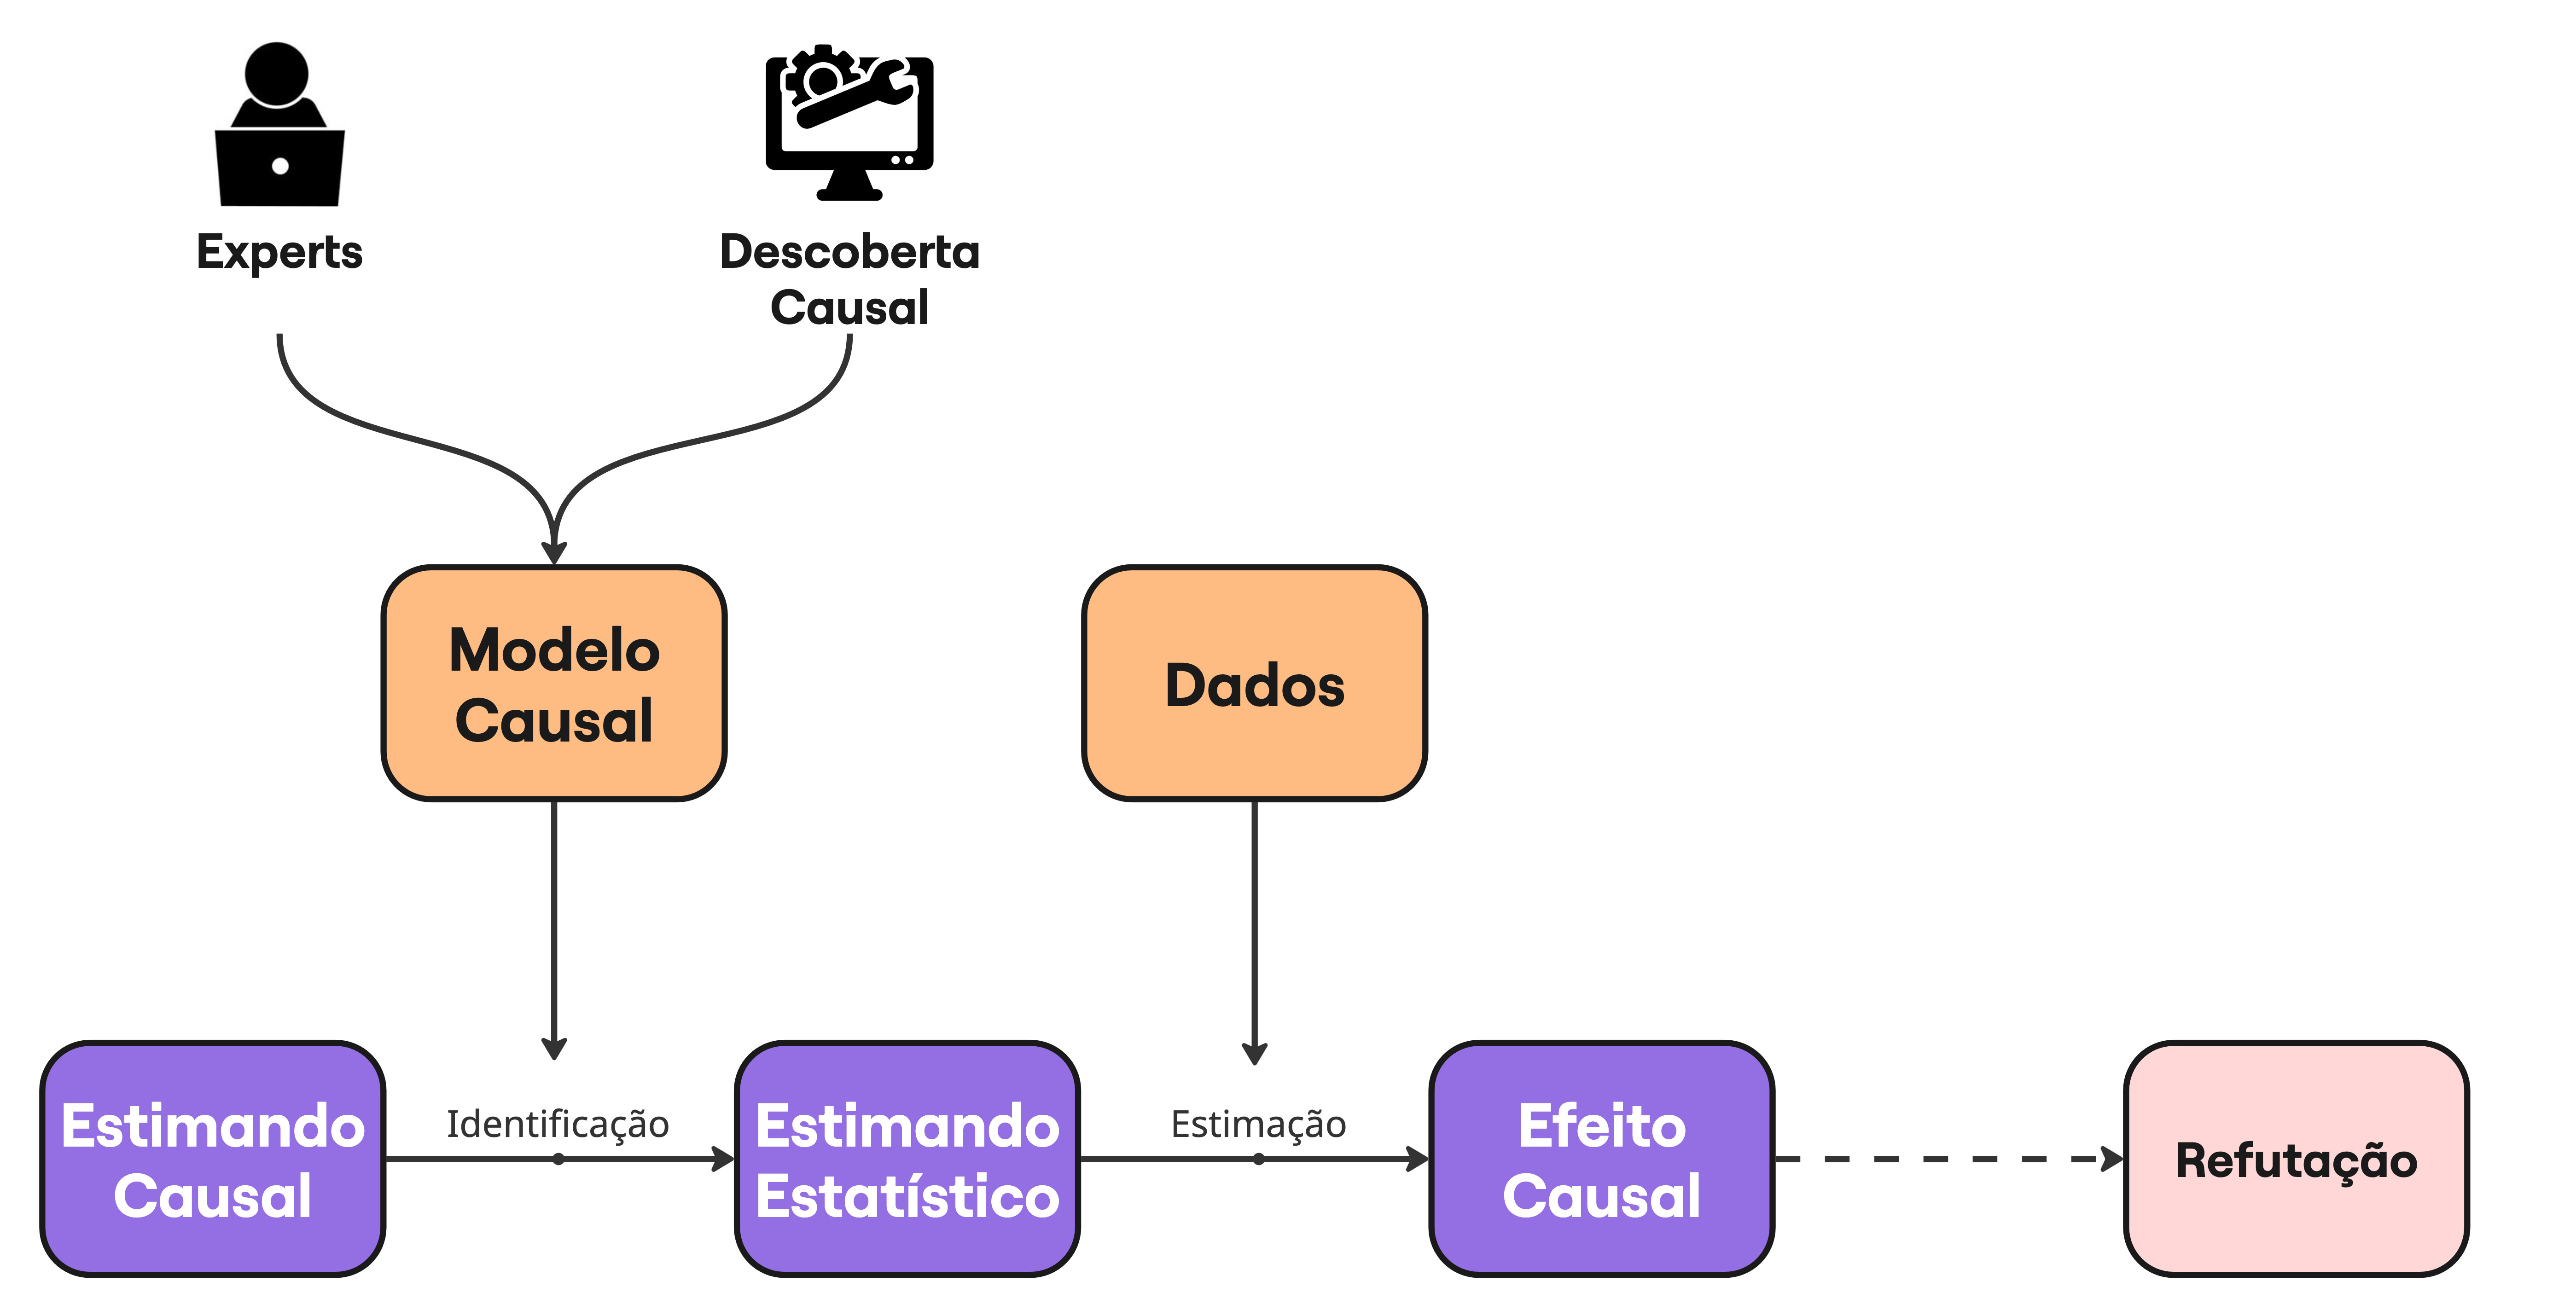
\includegraphics[width=0.5\textwidth]{figures/causal_inference_flow.jpg}
    \end{figure}

    \pause
    Sem dataset de gabarito pra validar automaticamente, alguém precisa olhar o grafo e dizer ``faz sentido'' ou ``essa seta tá errada''.
    
    \pause
    Na prática, CD quase sempre entrega uma sugestão, não uma resposta final. Um humano com conhecimento de domínio é necessário pra ter uma resposta causal válida de fato.
\end{frame}

\begin{frame}{Quer dizer que é inútil sem um especialista?}
    \begin{figure}
        \centering
        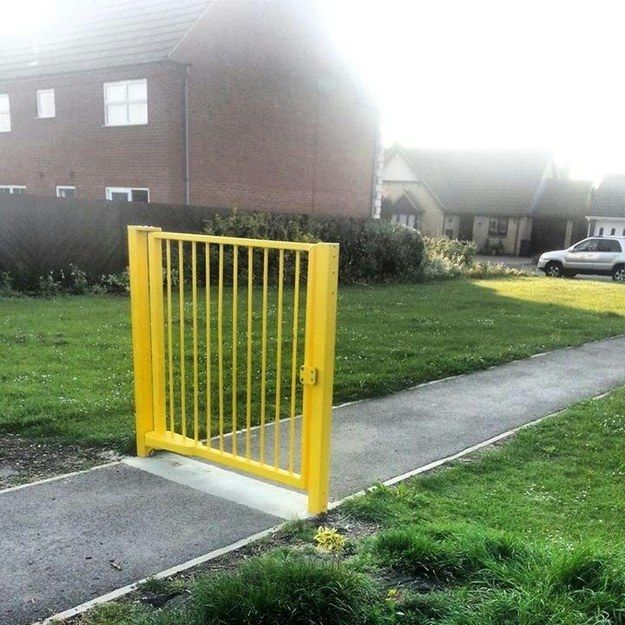
\includegraphics[width=0.22\textwidth]{figures/useless.jpg}
    \end{figure}

    \pause
    \texttt{\Large{NÃO!}}

    Mesmo sem um especialista, a análise automatizada de causalidade pode ser útil para melhorar a compreensão do problema, gerar hipóteses, e até mesmo melhorar modelos preditivos.

    \pause

    Afinal, modelos baseados apenas em correlação não são úteis?
\end{frame}

\begin{frame}{Mão na massa}
	\notebooklink{4}{4\_causal\_feature\_selection.ipynb}
\end{frame}